\documentclass[unicode,aspectratio=169,11pt]{beamer}
\usepackage{amsmath, amssymb, amsthm, color, latexsym, mathrsfs, bm}
\usefonttheme{professionalfonts}
\usepackage{luatexja}
\usepackage[ipaex]{luatexja-preset}
\renewcommand{\kanjifamilydefault}{\gtdefault}

\usetheme[
  sectionpage=none,
  numbering=fraction,
  block=fill
  ]{metropolis}

\title{
    The AI economist:
    Improving Equality and Productivity with AI-Driven Tax Policies
}
\subtitle{Stephan Zheng, Alexander Trott, Sunil Srinivasa, Nikhil Naik, Melvin Gruesbeck, David C. Parkes, and Richard Socher, 2020, mimeo.}
\author{Presenter: Yoji Tomita}
\date{RL-GTゼミ June 17, 2021}

\begin{document}

\maketitle

\begin{frame}{Table of Contents}
    \tableofcontents
\end{frame}

\section{1. Introduction}
\begin{frame}{1. Introduction}
    \begin{itemize}
        \item イントロダクション
    \end{itemize}
\end{frame}

\section{2. Economic Simulations: Learning in Gather-and-Build Games}

\begin{frame}{2. Economic Simulations: Learning in Gather-and-Build Games}{}
    \begin{itemize}
        \item Economic environmentについて.
        \item まずは税の無い設定("free-market")で説明する.
    \end{itemize}
\end{frame}

\subsection{2.1 Notation and Preliminaries}
\begin{frame}{2.1 Notation and Preliminaries}
    \begin{itemize}
        \item Partial-observable multi-agent Markov Games(MGs): $(S, A, r, \mathscr{T}, \gamma, o, \mathscr{I})$
        \begin{itemize}
            \item $S$ : 状態空間(state space)
            \item $A$ : 行動空間(action space)
            \item $r_{i,t}$ : 報酬関数(reward function)
            \item $\mathscr{T}$ : 遷移関数(transition function)  $s_{t+1} \sim \mathscr{T}(\cdot \mid s_t, \bm{a}_t)$
            \item $\gamma$ : 割引因子(discount factor)
            \item $o_{i,t}$ : 観測(observation)
            \item time step $t = 0, 1, \dots, H$.
        \end{itemize}
    \end{itemize}
\end{frame}

\begin{frame}{}{}
\begin{itemize}
    \item Agents' policy : $\pi_i(\cdot \mid o_{i,t}, h_{i,t}; \theta_i)$
    \begin{itemize}
        \item $h_{i,t}$ : hidden state(自分の私的情報と, 過去のhistory)
        \item $\theta_i$ : policyのparameter
        \item エージェント $i$ は次の最大化問題を得くpolicyを求める:
        \[
            \max_{\theta_i} \mathbb{E}_{a_i \sim \pi_i, \bm{a}_{-i} \sim \bm{\pi}_{-i}, s'\sim \mathscr{T}}\left[\sum_{t}\gamma^t r_{i,t}\right].
            \tag{1}
        \]
    \end{itemize}
     
    \item データ効率性のため, すべてのエージェントはtrainingの間パラメータ$\theta$を共有する.
    \item 彼らの行動 $\pi_i(a_i\mid o_i, h_i; \theta)$ は, agent-specific observations $o_i$ と hidden-state $h_i$によって異なる.
\end{itemize}
\end{frame}

\subsection{2.2 Environment Rules and Dynamics}
\begin{frame}{2.2 Environment Rules and Dynamics}{}
{\bf Gather-and-Build game}
\begin{itemize}
    \item 2次元のgrid ($25 \times 25$) からなる世界が舞台.
    \item エージェントはフィールドを歩き回り, 資源(石と木)を集め, それらを1つずつ使って家を建て, また資源をcoinを介してトレードする.
    \item 資源は空タイルに確率的に産み出される.
    \item エージェントは家を建てるとcoinが得られるが, 得られるcoinはagentのskillごとに異なる.
\end{itemize}
\end{frame}

\begin{frame}{}{}
{\bf Labor and Skill.}
\begin{itemize}
    \item Agentのaction(moving, gathering, trading, building)にはそれぞれlabor costが設定されている.
    \item 各timeにagentがどれか1つ行動をとると, そのlabor costがかかる.\\
     
    \item building skill (1以上3以下)が各agentに設定されていて, 家を建てるとagentは $10 \times$ skill 分のcoinを得る.
    \item collection skill (1以上2以下)もあり, 資源を拾うとこのskill分の資源を得る\\
          (skill 1.2 の場合, 確定で1つ資源を得て, さらに確率0.2でもう1つ資源を得る)
\end{itemize}
\end{frame}

\begin{frame}{}{}
{\bf Environment Scenario.}
\begin{columns}[t]
    \begin{column}{0.6\textwidth}
        \begin{itemize}
            \item fieldは水により4つの区域に別れている(水部分は通れない)
            \item 資源は空間的に集まって発生する.
            \item 4 agents
            \item buildng skills は 1.13, 1.33, 1.65, 22.2(Pareto分布 w/ exponent $a=4$, scale $m=1$のquartilesを元に設定)
            \item 1 episodeは$H = 1000$ time stepsからなる.
        \end{itemize}
    \end{column}
    \begin{column}{0.4\textwidth}
        \begin{center}
            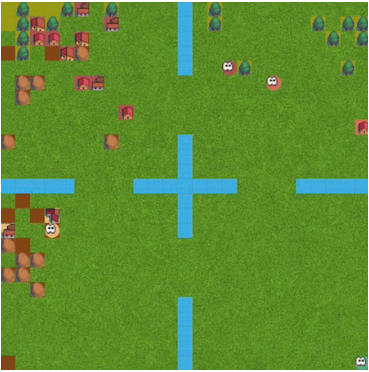
\includegraphics[width=5cm]{figure1.png}
        \end{center}
    \end{column}
\end{columns}
\end{frame}

\subsection{2.3 Using Machine Learning to Optimize Agent Behavior}
\begin{frame}{2.3 Using Machine Learning to Optimize Agent Behavior}{}
    \begin{itemize}
        \item Agentのutility function:
        \[
            u_i(x_{i,t}, l_{i,t}) = \mathrm{crra}\left(x_{i,t}^c \right) - l_{i,t},
            \ \ \ \mathrm{where}\ \ \mathrm{crra}(z) = \frac{z^{1-\eta} - 1}{1-\eta},\ \ \eta>0.
            \tag{2}
        \]
        \begin{itemize}
            \item $x_{i,t} = (x_{i,t}^w, x_{i,t}^s, x_{i,t}^c)$: $i$の保有する木・石・コイン.
            \item $l_{i,t}$: 蓄積労働量.
            \item $\eta$: エージェントのutility functionのnon-linearityをコントロールするパラメータ.
        \end{itemize}
        \item Rational economic agentは以下の最大化を行う.
        \[
            \forall i : \max_{\pi_i} \mathbb{E}_{a_i \sim \pi_i,\ \bm{a}_{-i}\sim \bm{\pi}_{-i}, s'\sim \mathscr{T}}
            \left[u_i(x_{i,0}, l_{i,0}) + \sum_{t=1}^H\gamma^t \underbrace{\left(u_i(x_{i,t}, l_{i,t})-u_i(x_{i,t-1}, l_{i,t-1})\right)}_{=r_{i,t}}\right].
            \tag{3}
        \]
    \end{itemize}
\end{frame}

\begin{frame}{}{}
{\bf Deep RL agents}
\begin{itemize}
    \item deep neural networkを用いるagent policyをmodellingする:
    \[ a_{i,t} \sim \pi(o^{\mathrm{world}}_{i,t}, o^{\mathrm{agent}}_{i,t}, o^{\mathrm{market}}_{i,t}, o^{\mathrm{tax}}_{i,t}, h_{i,t-1};\theta) \]
    \begin{itemize}
        \item $o^{\mathrm{world}}_{i,t}$: 近くの状況に関する観測.
        \item $o^{\mathrm{agent}}_{i,t}$: publicなagentの状況(資源・コイン保有)と, private agent states(skill値とlabor performed)
        \item $o^{\mathrm{market}}_{i,t}$: transfer marketの状況(bid, ask offer)
        \item $o^{\mathrm{tax}}_{i,t}$: tax rates
    \end{itemize}
\end{itemize}
\end{frame}

\end{document}